\documentclass[a4paper,14pt]{article}
\usepackage[14pt]{extsizes}




\usepackage{cmap}					% поиск в PDF
\usepackage{mathtext} 				% русские буквы в формулах
\usepackage[T2A]{fontenc}			% кодировка
\usepackage[utf8]{inputenc}			% кодировка исходного текста
\usepackage[english,russian]{babel}	% локализация и переносы
\usepackage{ulem}                   % зачеркнутый текст
\usepackage{amssymb}			% пакет математики
\usepackage{float}
\usepackage{amsmath}
\usepackage{graphicx}
\DeclareGraphicsExtensions{.png}

%%% Страница
%\usepackage{extsizes} % Возможность сделать 14-й шрифт
\usepackage[left=1cm,right=1cm,top=1cm,bottom=1cm]{geometry} % Простой способ задавать поля
\pagestyle{empty}

\begin{document}


\begin{center}
ФЕДЕРАЛЬНОЕ ГОСУДАРСТВЕННОЕ ОБРАЗОВАТЕЛЬНОЕ БЮДЖЕТНОЕ УЧРЕЖДЕНИЕ ВЫСШЕГО ОБРАЗОВАНИЯ

    \textbf{«ФИНАНСОВЫЙ УНИВЕРСИТЕТ ПРИ ПРАВИТЕЛЬСТВЕ РОССИЙСКОЙ ФЕДЕРАЦИИ»}

Факультет информационных технологий и анализа больших данных

Департамент анализа данных и машинного обучения

\textit{
	\textbf{Дисциплина: «Теория вероятностей и математическая статистика»}}

\textit{Направление подготовки: 01.03.02 «Прикладная математика и информатика»}

\textit{Профиль: «Анализ данных и принятие решений в экономике и финансах»}

\textit{Форма обучения очная, учебный 2020/2021 год, 4 семестр}

\textbf{Билет 122}

\end{center}

\begin{enumerate}


\item


Сформулируйте определение случайной выборки из конечной генеральной совокупности. Какие
виды выборок вам известны? Перечислите (с указанием формул) основные характеристики выборочной и генеральной совокупностей




Здесь очень много исчерпывающей информации о выборках из генеральной совокупности и про различные виды выборок


\item



Случайные величины $X$ и $Y$ независимы и имеют равномерное
распределение на отрезках $[0;2]$ и $[0;8]$ соответственно. Для случайной величины $Z=\frac{Y}{X}$ найдите: 
1) функцию распределения $F_Z(x)$;
2) плотность распределения $f_Z(x)$ и постройте график плотности;
3) вероятность $\P(2,\!016\leqslant Z\leqslant 6,\!716)$.




%\folder 2_53d24.png
1) Функция распределения $F_Z(x)$ имеет вид:
$
F_Z(x)=\left\{
\begin{array}{l}
0, x\leqslant 0;\\
\frac{x}{8}, 0\leqslant x\leqslant 4\approx 4,\!0;\\
1 - \frac{2}{x}, x\geqslant4;
\end{array}.
\right.
$
2) Плотность распределения $f_Z(x)$ имеет вид:
$
f_Z(x)=\left\{
\begin{array}{l}
0, x<0;\\
\frac{1}{8}, 0\leqslant x\leqslant 4\approx 4,\!0;\\
\frac{2}{x^{2}}, x\geqslant4;
\end{array}.
\right.
$


\begin{figure}[H]
    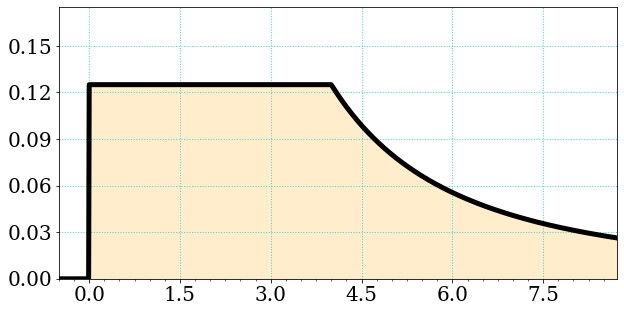
\includegraphics[width=0.9\textwidth]{2_53d24}
\end{figure}


3) вероятность равна:
$
\P(2,\!016\leqslant Z\leqslant 6,\!716)=
0,\!4502.
$


\item

    
	Случайная величина Y принимает только значения из множества $\{2, 1\}$, при этом $P(Y=2) = 0.61$.
	Распределение случайной величины X определено следующим образом:
	\begin{equation*}
		X | Y =
		\begin{cases}
			$8$ * y, с вероятностью $ 0.15$ \\
			$6$ * y, с вероятностью $ 1 - 0.15$
		\end{cases}
	\end{equation*}

	Юный аналитик Дарья нашла матожидание и дисперсию $X$.

	Помогите Дарье найти матожидание и дисперсию величины $X$
	


	

	Первым этапом надо найти характеристики случайной величины $Y$

	$E(Y) = 2 * 0.61 + 1 * (1 - 0.61)$

	$Var(Y) = E(Y^2) - [E(Y)]^2 = 2^2 * 0.61 + 1^2 * (1 - 0.61) - [E(Y)]^2$


	Перейдем к рассмотрению характеристик условной случайно величины X

	$E(X) = E(E(X|Y)) = E[E(8 * Y) * 0.15 + E(6 * Y) * (1 - 0.15)] = E(Y) * (8 * 0.15 + 6 * (1 - 0.15)) = 10.143$

	$E(Var(X|Y)) = E[b * Var(c3 * Y) + (1 - b) * Var(c4 * Y)] = Var(Y) * (c3^2 * b + c4^2 * (1- b)) $

	$Var(E(X|Y)) = E(X^2|Y) - [E(X)]^2 = [E(Y)]^2 * (b * c3^2 + (1-b)*c4^2) - E(X)]^2$

	$Var(X) = E(Var(X|Y)) + Var(E(X|Y)) = 10.88555$
	

\item

    
    Создайте эмперические совокупности  $\mathtt{\text{sin}}$ и $\mathtt{\text{cos}}$ вида $\mathtt{\text{sin}}(1),\mathtt{\text{sin}}(2), ..., \mathtt{\text{sin}}(60) $ и $\mathtt{\text{cos}}(1),\mathtt{\text{cos}}(2), ..., \mathtt{\text{cos}}(60). $

    Найдите эмпирическое среднее и эмпирическое стандартное отклонение совокупности $\mathtt{\text{sin}}$, её четвёртый эмпирический центральный момент и эмпирический эксцесс.

    Кроме того, найдите эмпирический коэффициент корреляции признаков $\mathtt{\text{sin}}$ и $\mathtt{\text{cos}}$ на совокупности натуральных чисел от $1$ до $60$.
    


    
    Используя

	$E(X) = sum(X) / n$

	$Var(X) = E(X^2) - [E(X)]^2$

	$\mu_4(X) = E((X-E(X))^4)$

	$Ex = \frac{\mu_4(X)}{[\sigma(X)]^4} - 3$

	$r_{xy} = \frac{E(XY) - E(X) * E(Y)}{\sigma(X) * \sigma(Y)}$

    рассчитаем искомые значения.

    Ответы: $0.02724, 0.70603, 0.37291, -1.49926, 0.00012$.

    

\item


(10) Эмпирическое распределение признаков $X$ и $Y$ на генеральной совокупности $\Omega$ задано таблицей частот  
 
\begin{tabular}{ | c | c | c | c | }
\hline
 & $Y = 2$ & $Y = 4$ & $Y = 5$  \\ \hline
$X = 200$ & $11$ & $26$ & $27$\\ \hline
$X = 300$ & $5$ & $10$ & $21$\\
\hline
\end{tabular}

Из $\Omega$ случайным образом без возвращения извлекаются $6$ элементов. 
Пусть $\bar X$ и $\bar Y$ – средние значения признаков на выбранных элементах. 
Требуется найти: 1) математическое ожидание $\mathbb{E}(\bar Y)$; 2) стандартное отклонение $\sigma(\bar X)$ ; 
3) ковариацию $Cov(\bar X, \bar Y)$




1) математическое ожидание $\mathbb{E}(\bar Y)$: $4.16$ 
2) стандартное отклонение $\sigma(\bar X)$: $233.542$
3) ковариацию $Cov(\bar X, \bar Y)$: $0.4975$


\item

    
	Известно, что доля возвратов по кредитам в банке имеет распределение $F(x) = x^{\beta}, 0 \le x \le 1$. Наблюдения показали, что в среднем она составила $62.0$\%. Методом моментов оцените параметр $\beta$ и вероятность того, что она опуститься ниже $59.0$\%.
	


	

	$f(x) = F'(x) = \beta \cdot x^{\beta - 1}$

	$\mu_{1} = E(X) = \int_{-\inf}^{\inf}x \cdot f(x) = \int_{-\inf}^{\inf} \beta \cdot x^{\beta} = \beta \cdot \frac{x^{\beta + 1}}{\beta + 1}\bigg|_0^1 = \frac{\beta}{\beta + 1}$

	$\beta = (\beta + 1) \cdot 62.0$

	$\beta = \frac{62.0}{1 - 62.0}$

	$ P(x \le 59.0) = F(59.0) = 59.0^{1.63} $

    Ответ: $1.63, 0.42$
	

\end{enumerate}

\begin{figure}[H]
	Подготовил
	\hfill
	
\includegraphics[width=2cm]{Prepared}
	П.Е. Рябов
\end{figure}


\begin{figure}[H]
	Утверждаю:\\
	Первый заместитель\\
	руководителя департамента\\
	Дата 01.06.2021
	\hfill
	
\includegraphics[width=2cm]{Approved}
	Феклин В.Г.
\end{figure}

\end{document}

